\chapter{Исследовательская часть}

В этой части приведены технические характеристики устройства,
на котором проводилось исследование быстродействия программы, и результаты исследования.

\section{Технические характеристики}

Спецификации устройства, использованного для тестирования:
\begin{itemize}[label=--]
	\item оперативная память 16 ГБ;
	\item процессор Intel(R) Core(TM) i7-9750H с тактовой частотой 2.60 ГГц;
	\item операционная система Windows 10 Домашняя 64-разрядная с версией 22H2.
\end{itemize}

Устройство было нагружено только встроенными приложениями и подключено в сеть электропитания. 

\section{Проведение исследования}

Целью исследования является определение зависимостей: 
\begin{itemize}[label=--]
	\item времени визуализации сцены от количества полигонов;
	\item времени визуализации сцены от количества примитивов;
	\item времени визуализации сцены от размера примитива.
\end{itemize}

По результатам исследования должны быть составлены таблицы и построены графики зависимости.

\subsection{Зависимость времени визуализации от количества полигонов}

Исследование проводится с использованием многогранника, где каждая грань соответствует отдельному полигону. Для визуализации сцены выбран <<теневой>> режим, так как он является наиболее ресурсоемким из доступных в программе.

Для каждого многогранника время визуализации измеряется трижды, после чего вычисляется среднее значение. Все замеры производятся в секундах.

Результаты определения зависимости времени визуализации сцены от количества полигонов приведены в таблице~\ref{tbl:research1}.

\begin{table}[h]
	\centering
	\caption{Зависимость времени визуализации сцены от количества полигонов}
	\begin{tabular}{|c|c|}
		\hline
		\textbf{Количество полигонов (шт.)} & \textbf{Время визуализации (сек.)} \\
		\hline
		10  & 5,01 \\
		20  & 7,40 \\
		30  & 8,37 \\
		40  & 8,73 \\
		50  & 9,13 \\
		60  & 9,55 \\
		70  & 10,00 \\
		80  & 10,38 \\
		90  & 10,85 \\
		100 & 11,29 \\
		\hline
	\end{tabular}
	\label{tbl:research1}
\end{table}

По таблице~\ref{tbl:research1} был построен график~\ref{fig:research1}, который наглядно демонстрирует результаты определения зависимости времени визуализации сцены от количества полигонов. Исходя из графика можно сделать вывод, что данная зависимость близка к линейной.

\clearpage

\begin{figure}[h] 
	\centering
	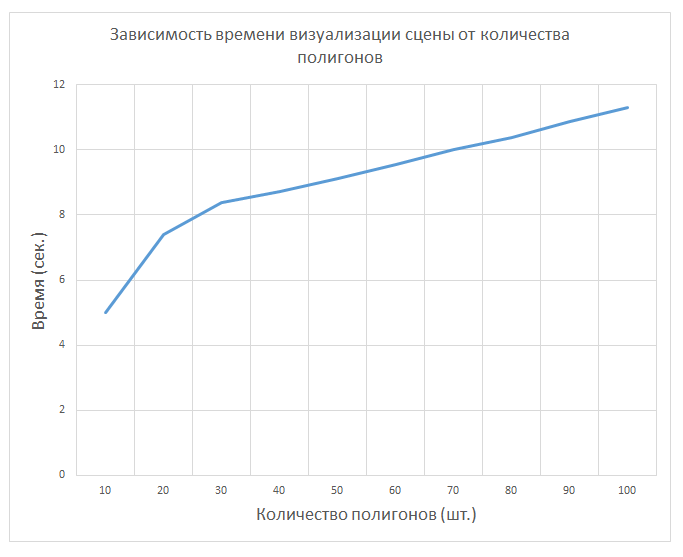
\includegraphics[width=1\textwidth]{images/research1.png}
	\caption{Зависимость времени визуализации сцены от количества полигонов} 
	\label{fig:research1} 
\end{figure}

\subsection{Зависимость времени визуализации от количества примитивов}

Исследование проводится с использованием многогранников, имеющих 3, 6 и 9 граней. Для визуализации сцены выбран <<теневой>> режим, так как он является наиболее ресурсоемким из доступных в программе.

Для каждого многогранника время визуализации измеряется трижды, после чего вычисляется среднее значение. Все замеры производятся в секундах.

\section{Вывод}

<что сделали и получили в результате, кратко>

\clearpage
